\documentclass[border=6pt]{standalone}
% Shared style for the methodology figures, after the block diagrams of
% "Attention Is All You Need": rounded blocks in soft colours with fine outlines,
% a grey container with a repetition count, and thin arrows.
\usepackage{libertinus}
\usepackage{amsmath}
\usepackage{xcolor}
\usepackage{tikz}
\usetikzlibrary{positioning,arrows.meta,calc,fit,backgrounds,shapes.geometric}

\definecolor{ink}{HTML}{1E2227}
\definecolor{muted}{HTML}{5C6670}
\definecolor{cRGB}{HTML}{2F6DB5}
\definecolor{cIR}{HTML}{C0622B}
\definecolor{cFuse}{HTML}{3B8B66}
\definecolor{cTime}{HTML}{7450A8}
\definecolor{cNeutral}{HTML}{66707B}
\definecolor{cData}{HTML}{8C6A2F}
\definecolor{cAlert}{HTML}{A8384A}
\definecolor{cHead}{HTML}{B08A2E}
\color{ink}

\tikzset{
  blk/.style   = {rounded corners=3pt, align=center, font=\small, inner xsep=6pt, inner ysep=4.5pt,
                  minimum height=0.8cm, line width=0.5pt, text=ink,
                  execute at begin node={\hyphenpenalty=10000}},
  vis/.style   = {blk, fill=cRGB!14, draw=cRGB!65},
  thr/.style   = {blk, fill=cIR!15, draw=cIR!65},
  fus/.style   = {blk, fill=cFuse!16, draw=cFuse!70},
  scn/.style   = {blk, fill=cTime!14, draw=cTime!65},
  neu/.style   = {blk, fill=cNeutral!10, draw=cNeutral!55},
  hed/.style   = {blk, fill=cHead!16, draw=cHead!70},
  dat/.style   = {blk, fill=cData!12, draw=cData!60},
  io/.style    = {align=center, font=\small, text=ink},
  op/.style    = {circle, draw=cNeutral!70, fill=white, line width=0.5pt, inner sep=0pt,
                  minimum size=5.2mm, font=\small},
  lab/.style   = {font=\footnotesize\itshape, text=muted, align=center},
  note/.style  = {font=\footnotesize, text=muted, align=left},
  ar/.style    = {-{Stealth[length=2.1mm,width=1.6mm]}, line width=0.55pt, draw=ink!75},
  dar/.style   = {ar, dash pattern=on 2.4pt off 1.6pt},
  gar/.style   = {ar, draw=cData, dash pattern=on 2.4pt off 1.6pt},
  box/.style   = {rounded corners=6pt, fill=cNeutral!5, draw=cNeutral!45, line width=0.5pt},
  over/.style  = {preaction={draw=white, line width=3.2pt, -}},
}

\begin{document}
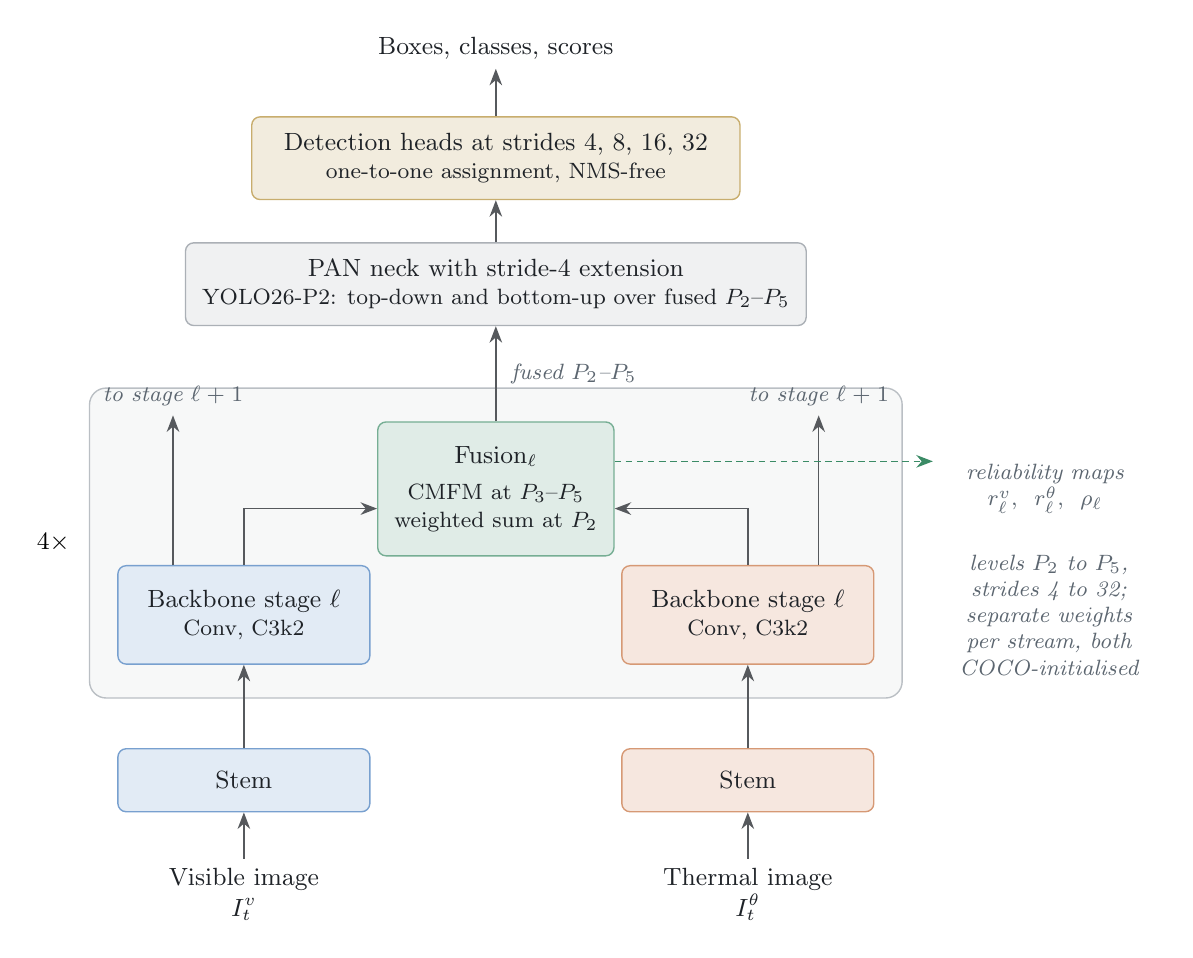
\begin{tikzpicture}[node distance=6mm]
  \node[io] (iv) at (0,0) {Visible image\\ $I^{v}_{t}$};
  \node[io] (it) at (6.4,0) {Thermal image\\ $I^{\theta}_{t}$};
  \node[vis, minimum width=3.2cm] (sv) at (0,1.45) {Stem};
  \node[thr, minimum width=3.2cm] (st) at (6.4,1.45) {Stem};
  \draw[ar] (iv) -- (sv); \draw[ar] (it) -- (st);

  \node[vis, minimum width=3.2cm, minimum height=1.25cm] (bv) at (0,3.55) {Backbone stage $\ell$\\[-1pt] \footnotesize Conv, C3k2};
  \node[thr, minimum width=3.2cm, minimum height=1.25cm] (bt) at (6.4,3.55) {Backbone stage $\ell$\\[-1pt] \footnotesize Conv, C3k2};
  \node[fus, minimum width=2.6cm, minimum height=1.7cm] (fu) at (3.2,5.15)
       {Fusion$_\ell$\\[2pt] \footnotesize CMFM at $P_3$--$P_5$\\[-1pt] \footnotesize weighted sum at $P_2$};
  \draw[ar] (sv) -- (bv); \draw[ar] (st) -- (bt);
  \draw[ar] (bv.north) |- ($(fu.west)+(0,-0.25)$);
  \draw[ar] (bt.north) |- ($(fu.east)+(0,-0.25)$);
  \draw[ar] ($(bv.north)+(-0.9,0)$) -- ++(0,1.9) node[lab, above, text width=2.3cm] {to stage $\ell+1$};
  \draw[ar] ($(bt.north)+(0.9,0)$) -- ++(0,1.9) node[lab, above, text width=2.3cm] {to stage $\ell+1$};

  \begin{scope}[on background layer]
    \node[box, fit=(bv)(bt)(fu), inner xsep=10pt, inner ysep=12pt] (rep) {};
  \end{scope}
  \node[font=\small, anchor=east] at ($(rep.west)+(-0.12,0)$) {$4\times$};
  \node[lab, anchor=west, text width=2.7cm] at (8.75,3.55)
       {levels $P_2$ to $P_5$, strides 4 to 32; separate weights per stream, both COCO-initialised};

  \node[neu, minimum width=6.2cm, minimum height=1.05cm] (nk) at (3.2,7.75)
       {PAN neck with stride-4 extension\\[-1pt] \footnotesize YOLO26-P2: top-down and bottom-up over fused $P_2$--$P_5$};
  \node[hed, minimum width=6.2cm, minimum height=1.05cm] (hd) at (3.2,9.35)
       {Detection heads at strides 4, 8, 16, 32\\[-1pt] \footnotesize one-to-one assignment, NMS-free};
  \node[io] (out) at (3.2,10.75) {Boxes, classes, scores};
  \draw[ar] (fu) -- node[lab, right=2pt] {fused $P_2$--$P_5$} (nk);
  \draw[ar] (nk) -- (hd); \draw[ar] (hd) -- (out);

  \node[lab, anchor=west, text width=2.6cm] (rho) at (8.75,5.15) {reliability maps\\ $r^{v}_\ell,\; r^{\theta}_\ell,\; \rho_\ell$};
  \draw[dar, draw=cFuse] (fu.east) ++(0,0.35) -- (rho.west |- 0,5.5);
\end{tikzpicture}
\end{document}
